\section{Nebulas Rank}
\label{sec:rank}

\subsection{Introducción a Nebulas Rank} \label{subsec:value}
Actualmente la tecnología blockchain y su comunidad han crecido hasta llegar a ser un ecosistema a gran escala. Sin embargo, la percepción popular de blockchain en el mundo es todavía algo superficial; no existe aún una forma razonable de evaluar el valor de una entidad (tal como la dirección de un usuario) en el blockchain. Por ende, trabajamos para elaborar una medida universal de valor. Mediante la exploración y el uso de actividades en el blockchain, hemos creado \textbf{Nebulas Rank} un algoritmo a través del cual se puede cuantificar el valor de cada entidad (como la dirección de un usuario). \textbf{Nebulas Rank} está diseñado para:\begin{itemize}
	\item servir como una medida nativa de valor y como un algoritmo central para distintos escenarios fundamentales, como el algoritmo de consenso (véase \refsec{sec:pod}), el Protocolo de Incentivos a Desarrolladores (véase \refsec{sec:dip}) y el motor de búsquedas de blockchain (véase \refsec{sec:search}), entre otros;
	\item inspirar valuaciones diversas y percepciones más profundas en el ecosistema blockchain, de modo de guiar con más precisión las decisionesde negocios y las actividades de investigación.
\end{itemize}
Basándonos en las metas arriba mencionadas, podemos definir la medición de valor de \textbf{Nebulas Rank} desde tres \textit{dimensiones}:
\begin{itemize}

	\item \textbf{Liquidez}, la frecuencia y escala de las transacciones es la primera dimensión que mide \textbf{Nebulas Rank}. Las finanzas son esencialmente actividades que optimizan los recursos sociales a través de la liquidez del capital y que promueven el desarrollo económico. Blockchain establece una red de valor, en el sentido de que a mayor cantidad y escala de transacciones se logra una mayor liquidez, lo que aumenta aún más las transacciones y su escala, formando así un círculo virtuoso.

	\item \textbf{Propagación}, el alcance y la profundidad de la liquidez de los activos es la segunda dimensión que mide \textbf{Nebulas Rank}. En las redes sociales la propiedad de propagación —es decir: la velocidad, el alcance y la profundidad de la transmisión de la información— es un índice clave que muestra la calidad de la red y el crecimiento de los usuarios. El mismo patrón se puede observar en el mundo blockchain: una propagación de gran alcance implica una liquidez de activos más amplia y profunda, lo que mejora la calidad y la escala de los activos.

	\item \textbf{Interoperabilidad} es la tercera dimensión que mide textbf{Nebulas Rank}. Durante la primera etapa de Internet, sólo existían sitios web sencillos y la información estaba aislada. En la actualidad la información se puede enviar desde distintas plataformas y es cada vez más raro encontrar información aislada. Esta tendencia podría entenderse como un proceso de reconocimiento de la información desde una perspectiva dimensional superior. Creemos que el mundo blockchain también sigue un patrón similar, aunque su desarrollo es más rápido. Habrá más información disponible sobre los activos de los usuarios, sobre contratos inteligentes y sobre {\dapp}s. Y, además, todas esas entidades interactuarán con más frecuencia. Por lo tanto, es cada vez más importante que exista una mejor interoperabilidad en el blockchain.

\end{itemize}

Elegimos los registros de transacciones en blockchain como el origen de datos para \textbf{Nebulas Rank} debido a que la \textit{trayectoria} en el mundo de blockchain es más clara y confiable que la del mundo real. Los datos de las transacciones —como las transferencias y las llamadas a contratos inteligentes— quedan registradas en el blockchain. Aun así, no es trivial diseñar algoritmos de valuación para los datos de transacciones en el blockchain, ya que éstas son naturalmente anónimas y poseen una mayor escala de datos que en el mundo real.

A continuación se describen tres propiedades principales para \textbf{Nebulas Rank}:

\begin{itemize}

	\item Veracidad. Una entidad debe pagar un costo razonable para mejorar su valuación, lo que asegura que el algoritmo pueda identificar a los usuarios legítimos y valiosos. Por un lado, en escenarios como el algoritmo de consenso y el DIP, una valuación veraz anima a los usuarios a contribuir de manera honesta con el fin de obtener un \textit{feedback} positivo. Por otro lado, un resultado veraz proporciona una representación jerárquica significativa de todos los usuarios, lo que será útil para los responsables de tomar decisiones;

	\item Computabilidad. Al ser un indicador fundamental, es vital que el resultado de \textbf{Nebulas Rank} sea accesible instantáneamente, lo que requiere una baja complejidad computacional;

	\item Determinismo. Tal como es requerido en escenarios como el algoritmo de consenso y el DIP, el resultado del cálculo de \textbf{Nebulas Rank} debe ser idéntico y replicable en cualquier cliente.

\end{itemize}

A continuación, diseñamos el framework básico de \textbf{Nebulas Rank}. En primer lugar, los registros de transacciones se representan mediante grafos. En el grafo de transacción (grafo de entidades), cada nodo tiene una entidad asignada, y cada arista representa la transferencia entre dos entidades\cite{Tschorsch2015}. El grafo de transacciones encarna el hecho de que la transferencia de dinero entre usuarios conduce al flujo de activos, lo que ayuda a representar los conceptos de liquidez y propagación definidos anteriormente. Mientras tanto, la forma del grafo puede mostrar claramente la interoperabilidad entre los contratos. Mediante el grafo de transacciones derivado, clasificamos los nodos por su centralidad en la red. En el escenario de \textbf{Nebulas Rank}, LeaderRank \cite{Chen2013}\cite{Li2014} es una valuación más razonable que mejora lo ofrecido por PageRank de Google y NCDAwareRank de NEM \cite{nem}.

\subsection{Grafo de transacciones} \label{subsec:txg}
En esta subsección presentamos la forma en que derivamos los grafos de transacciones a partir de su historial.

Primero, para cualquier tiempo $t_0$, tomamos todas las transacciones \textbf{efectivas} entre direcciones individuales durante $[t_0- T, t_0]$ ($T$ es una constante, generalmente establecida en un mes), donde cualquier transacción puede ser representada como una 4-tupla $(s,r,a,t)$, con $s$ como la dirección de origen, $r$ como la dirección de destino, $a$ como el monto de la transferencia y $t$ como el tiempo de bloque. Decimos que una transacción será \textbf{efectiva} si $a>0$ y $s \neq r	$. Así, cualquier transacción \textbf{efectiva} durante $[t_0- T, t_0]$ se puede representar mediante un conjunto de 4-tuplas:

\begin{align}
\Theta(t_0) = \{(s, r, a, t)\ |\ t_0 - T \le t \le t_0\ \land \ a > 0 \land s \neq t \}
\end{align}

Basándonos entonces en $\Theta(t_0)$, construimos a grafo dirigido ponderado simple $G=(V,E, W)$, donde el conjunto de nodos, el conjunto de aristas y la ponderación de cada arista están denotadas por $V$, $E$ y $W$ respectivamente. Cada nodo en $V$ representa una dirección de cuenta individual, y cada arista en $E$ representa la intensidad de transferencias entre las dos direcciones. Las aristas son dirigidas y tienen asignadas las ponderaciones $w_e$ agregando los principales montos $K$ de todas las transacciones relacionadas:

\begin{align}\label{formula:edgeweight}
w_e = \sum_{i=1}^K a_i,\ s.t.\ a_i \in A_e
\end{align}
$A_e$ es un conjunto ordenado que comprende los montos de todas las transacciones desde $s$ hasta $r$ en $\Theta(t_0)$:
\begin{align}
A_e = \{a_i\ |\ e = (s,r) \land (s, r, a_i, t) \in \Theta(t_0) \land (a_i \ge a_j, \forall i \le j) \}
\end{align}

Adicionalmente, sea $N = |V|$, $M = |E|$, donde $|.|$ es el cardinal del conjunto. Para simplificar, cada nodo se representa por un número entero entre $1$ y $N$.

\begin{figure}[h]
\centering
	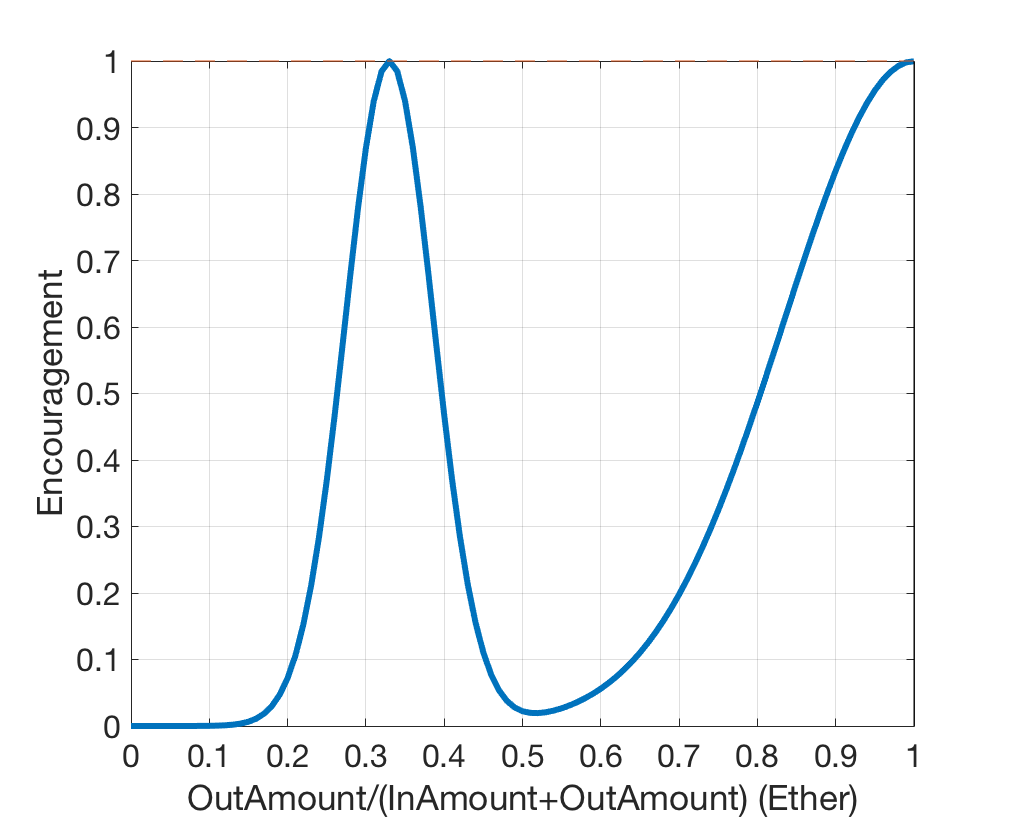
\includegraphics[width=0.55\textwidth]{figs/encouragement_en.png}
	\caption{Función de \textit{estímulo}}\label{fig:encouragement}
\end{figure}

Así, para cada nodo, de acuerdo a sus transferencias entrantes y salientes durante $[t_0\ —\ T,\ t_0]$, se computa la \textit{antigüedad de los depósitos} y se denota esta mediante $C_v$; basándonos en el monto total transferido y haciendo uso de la función \textit{estímulo} que se muestra en la \reffig{fig:encouragement}, se computa el valor \textit{estímulo} y se lo denota mediante $E_v$\footnote{La función estímulo se puede representar como una combinación lineal de dos distribuciones normales, que produce un valor máximo cuando la suma transferida es cero o alguna proporción de las transferencias de ingreso.}; úsense $C_v$ y $E_v$ de los nodos destino para reducir la ponderación de las aristas.

Finalmente, tómese el mayor componente débilmente conectado del grafo y manténganse aquellos nodos que pertenecen a ese componente. Los nodos eliminados reciben, por defecto, el menor puntaje de importancia.

La derivación de grafo descripta arriba contribuye a la propiedad de veracidad definida en \refsec{subsec:value}, cuya evidencia se ofrece en \refsec{subsec:robust}.

Usando el método descripto aquí, el grafo de transacción, donde $T$ representa 30 días y $K=2$, se genera basándonos en los datos transaccionales del blockchain principal de la red Ethereum, desde el bloque \#3629091(aproximadamente del primero de mayo de 2017) hasta el bloque \#3800775(de aproximadamente el 31 de mayo de 2017). Su visualización está disponible en la \reffig{fig:wgc}, y todos los nodos se redimensionan en función de su grado. Se puede observar que algunas casas de cambio famosas suelen interactuar con más cuentas que otras. Además, aún se desconocen las identidades de algunas direcciones que contribuyen con muchas transacciones.

\begin{figure}[htbp]
	\centering
	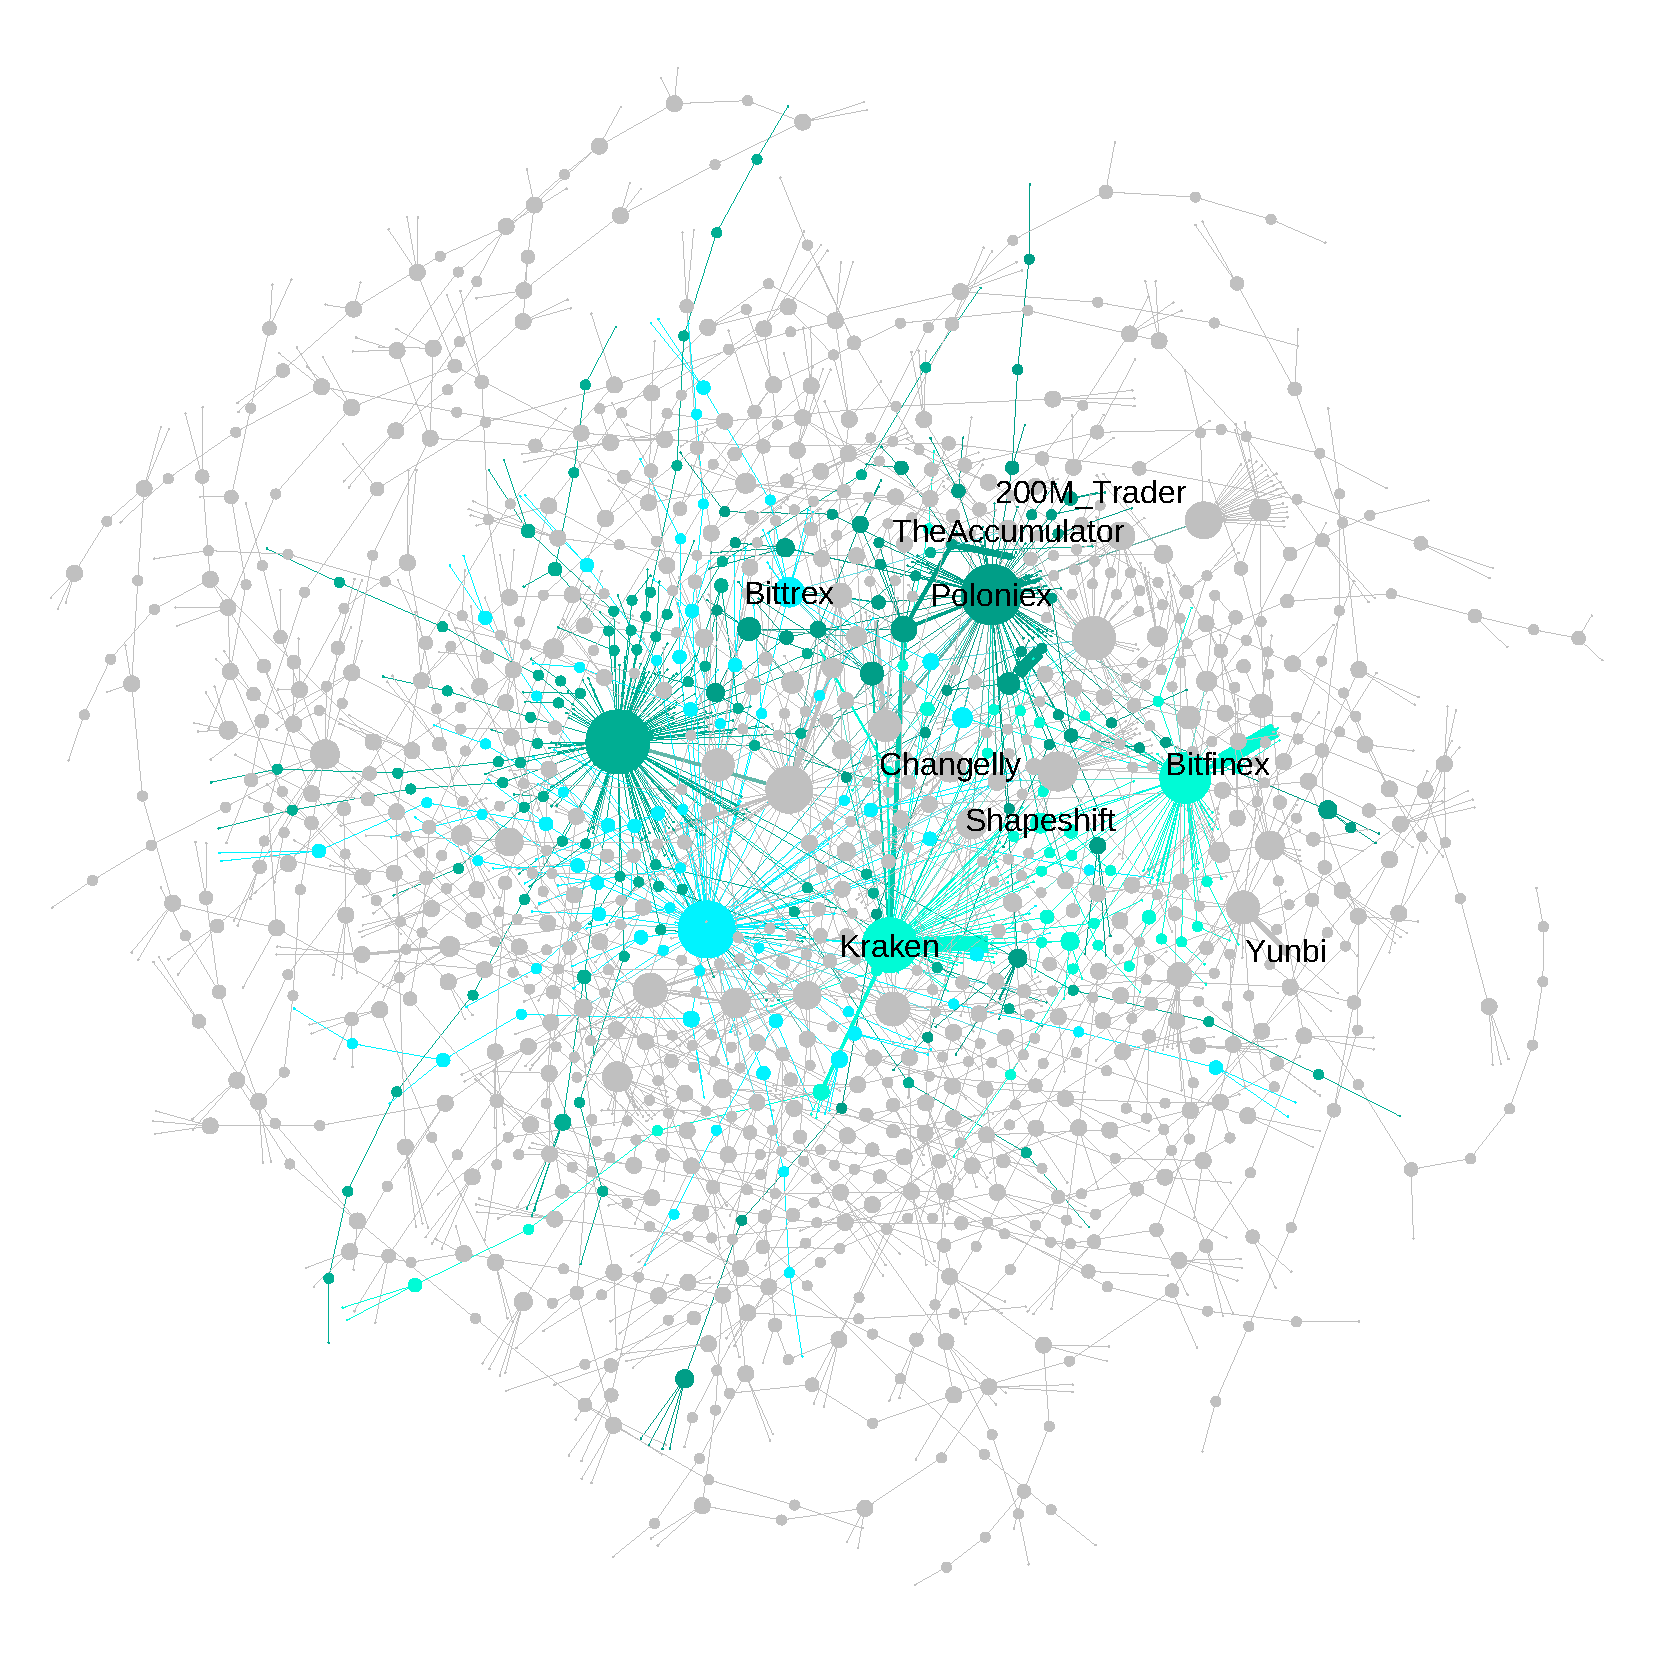
\includegraphics[width=0.85\textwidth]{figs/wgc1.png}
	\caption{Visualización del grafo de transacciones (parcial). \small{La gran escala de transacción (transferencia de capital) en la dirección significa un alto grado de entrada y salida en el nodo, representado por un gran diámetro en la figura. Algunos nodos están etiquetados con nombres, de acuerdo a Etherscan\cite{etherscan}}}\label{fig:wgc}
\end{figure}

\subsection{Algoritmo de valuación} \label{subsec:leaderrank}
Esta subsección explica cómo valuar nodos de acuerdo a su importancia en el grafo transaccional derivado.

Adoptamos LeaderRank\cite{Chen2013}\cite{Li2014} como el principal algoritmo. Primero, añadimos un nodo \textit{ground} con índice $0$ en el grafo de transacciones. Luego establecemos un vínculo bidireccional entre el nodo \textit{ground} $0$ y el resto de los nodos $i$ ($1 \leq i \leq N$), ponderando mediante la siguiente fórmula:
\begin{align}\label{formula:weight1}
w_{i,0} = \alpha( max\{ \sum_{w_{j,i} \neq 0} w_{j,i} - \sum_{w_{i,j} \neq 0} w_{i,j} , 0\} + \lambda C ), \forall i \in [1,N]
\end{align}
\begin{align}\label{formula:weight2}
w_{0,i}	= \beta ( \sum_{w_{i,m} \neq 0} w_{i,m} + \mu C), \forall i \in [1,N]
\end{align}
$C$ es la mediana del conjunto $\{w_{i,j} | w_{i,j} \neq 0, 0\leq i,j \leq N\}$, y $\alpha, \beta, \mu, \lambda$ son parámetros.

El esquema de ponderación puede explicarse de esta forma: los nodos con mayor cantidad de transferencias de ingresos obtienen aristas con mayor ponderación dirigidas desde el nodo \textit{ground}; los nodos con mayores transferencias absolutas (saldo resultante de restar los egresos a los ingresos) generan aristas con mayor ponderación, dirigidas al nodo \textit{ground}.

El esquema de ponderación puede explicarse de la siguiente manera: los nodos con más ingresos reciben aristas con más ponderación desde el nodo \textit{ground}; los nodos con mayores ingresos absolutos (ingresos menos egresos), generan aristas con mayor ponderación dirigidas al nodo \textit{ground}.

El proceso de cómputo de LeaderRank es similar al de PageRank, lo que puede ser entendido como el cálculo del estado de convergencia de un proceso de Markov. La única diferencia es que, luego de añadir el nodo \textit{ground}, ya no es necesario considerar el factor de amortiguación de PageRank\cite{Brin2010}\cite{page1999pagerank}. Esto es, luego de construir la matriz $H$ de acuerdo a la fórmula (\ref{formula:matrix}), el proceso de cómputo se itera hasta lograr convergencia, como se ve en la fórmula (\ref{formula:iteration}), con ajustes iniciales definidos por la fórmula (\ref{formula:init}). Finalmente, el puntaje de valuación del nodo \textit{ground} se distribuye uniformemente a todos los demás nodos, lo que produce la puntuación final para cada uno de ellos.
\begin{align} \label{formula:iteration}
	P^{t+1} = H \times P^{t}; P^1=[0, \frac{1}{N}, \frac{1}{N}, \dots, \frac{1}{N}]^T
\end{align}
\begin{align} \label{formula:matrix}
	h_{ij} = \frac{w_{(j,i)}}{\sum_k w_{(j,k)}}
\end{align}
\begin{align} \label{formula:init}
\forall v \in V, P^*_v \leftarrow P^*_v + \frac{P^*_{\mathcal{G}}}{N}
\end{align}

Suponemos que LeaderRank puede satisfacer la valuación y la propiedad algorítmica definida en \refsec{subsec:value}.
\begin{itemize}
	\item El resultado de LeaderRank puede ser entendido como el flujo en cada nodo dentro del equilibrio dinámico de una red de intercambio de dinero, lo que coincide con la valuación de \textbf{Nebulas Rank}: \textit{liquidez}, \textit{propagación} e \textit{interoperabilidad};
	\item El esquema de ponderación definido por las fórmulas (\ref{formula:weight2}) y (\ref{formula:weight1}) hace que sea más difícil de atacar (véase la discusión en \refsec{subsec:robust}), lo que satisface la propiedad de \textit{veracidad};
	\item LeaderRank puede ser calculado por iteración de potencia. Dado que la red es muy dispersa, la complejidad de la computación matricial no debería ser alta, lo que satisface las propiedades \textit{computable} y \textit{determinista}.
\end{itemize}


\subsection{Resistencia a la manipulación}\label{subsec:robust}
Veracidad, o resistencia a la manipulación, es la meta más desafiante y significativa de \textbf{Nebulas Rank}. Veamos algunos de los métodos posibles de manipulación:
\begin{enumerate}
	\item Bucle de transferencias: el atacante realiza transferencias sobre una topología de bucle, lo que permite que el mismo dinero circule sobre las mismas aristas repetidamente. Así, el atacante espera elevar la ponderación de las aristas asociadas;
	\item Transferencias a direcciones aleatorias, lo que espera lograr que el grado de egresos del nodo Sybil se incremente, y con ello la propagación de fondos;
	\item Formar un componente independiente de red con direcciones controladas por el atacante. Así, éste pretende ser un nodo central;
	\item Interactuar frecuentemente con direcciones de casas de cambio importantes, es decir, transferir el mismo dinero desde y hacia una o más direcciones de casas de cambio importantes, de modo de lograr una mejor posición estructural en la red.
\end{enumerate}

\textbf{Nebulas Rank} mitiga la manipulación a través de los siguientes mecanismos:
\begin{itemize}
	\item Gracias a las \textit{ventanas} móviles de $T$ bloques, el atacante no puede incrementar su valuación en el corto plazo;
	\item Dado que la ponderación de las aristas se decide por medio de las transacciones asociadas de mayor monto, transferir dinero a lo largo de una topología en bucle no incrementa ilimitadamente la ponderación de las aristas. Entretanto, de acuerdo al muestreo de datos en \refsec{subsec:txg}, $91\%$ de aristas corresponden a menos de dos transacciones, respectivamente. Así $K=2$ es una elección razonable para mantener la intensidad de la información de las aristas mientras se resiste la transferencia en bucle;
	\item Para lograr una mayor \textit{antigüedad en los depósitos}, el usuario necesita mantener el dinero en su dirección durante un cierto lapso de tiempo, lo que reduce la velocidad de este ataque;
	\item Con el fin de obtener el máximo valor de \textit{antigüedad de los depósitos}, tal como se ve en la \reffig{fig:encouragement}, la cuenta necesita enviar más de lo que ingresó o bien transferir sólo un pequeño porcentaje de sus ingresos; así, al intentar falsificar el flujo de dinero, el atacante verá reducirse rápidamente sus depósitos;
	\item A raíz de que sólo se seleccionan los componentes más grandes, otros componentes independientes —incluyendo el falsificado— quedarán filtrados. Según los datos de la muestra en \refsec{subsec:txg}, existen $453,285$ nodos y $970,577$ aristas, con $1,169$ componentes. En el componente más significativo, hay $449,746$ nodos, que representan $99.2\%$ del número total. En el segundo componente más significativo, hay sólo $133$ nodos, que representan $0.03\%$. Así, al seleccionar el componente más significativo, se mantiene gran parte de la actividad normal de la red mientras se filtran los componentes menores y las falsificaciones;
	\item Comparado a los algoritmos de valuación de sitios web tales como PageRank y NCDawareRank\cite{Nikolakopoulos2013}, el mecanismo definido por las \ref{formula:weight2} y \ref{formula:weight1} es más conservador en los nodos con pocos ingresos; esto es, los nodos con pocos ingresos obtienen enlaces más débiles con el nodo \textit{ground}. En el grafo de transacciones de blockchain es más probable que se generen nodos con bajos ingresos, y con sólo realizar transferencias a nodos aleatorios no basta para incrementar su grado de ingresos. De modo que \textbf{Nebulas Rank} puede incrementar la dificultad en realizar manipulaciones.
\end{itemize}

Luego, las siguientes conclusiones se basan en el grafo de transacciones de Ethereum en mayo de 2017.

Primero, algunas direcciones de \textbf{Nebulas Rank} se listan en la tabla \ref{table:nr}\footnote{Fuente del dominio: Etherscan\cite{etherscan}}. Puede observarse que las direcciones de las casas de cambio y algunas otras cuentas con un alto rendimiento de transacciones se valúan como nodos principales.

%\newpage
\begin{table}[!htbp]
\centering
\caption{\textbf{Las 10 direcciones principales} de \textbf{Nebulas Rank}, entre otras}
\label{table:nr}
\begin{tabular}{llllll}\toprule
\begin{tabular}[c]{@{}l@{}}Valuación\\ (Orden)\end{tabular} & Dirección                                                                                    & Nebulas Rank & Dominio          & Egreso (Ether) & Ingreso (Ether) \\
1  & \begin{tabular}[c]{@{}l@{}}0x267be1c1d684f78cb4f\\ 6a176c4911b741e4ffdc0\end{tabular} & 0.449275     & Kraken\_4   & 3214232.06  & 350008.00   \\
2  & \begin{tabular}[c]{@{}l@{}}0xd4c5867cec094721aab\\ c3c4d0fd2f2ac7878c79a\end{tabular} & 0.093798     &             & 58000.00    & 100947.00   \\
3  & \begin{tabular}[c]{@{}l@{}}0x027beefcbad782faf69f\\ ad12dee97ed894c68549\end{tabular} & 0.049277     & QuadrigaCX  & 207440.11   & 65606.40    \\
4  & \begin{tabular}[c]{@{}l@{}}0x0ee4e2d09aec35bdf08\\ 083b649033ac0a41aa75e\end{tabular} & 0.046831     &             & 56465.00    & 60087.96    \\
5  & \begin{tabular}[c]{@{}l@{}}0xc257274276a4e539741\\ ca11b590b9447b26a8051\end{tabular} & 0.037628     &             & 1071105.93  & 1434106.72  \\
6  & \begin{tabular}[c]{@{}l@{}}0xa53e0ca7d246a764993\\ f010d1fde4ad01189f4e6\end{tabular} & 0.033488     &             & 7764.68     & 3201.00     \\
7  & \begin{tabular}[c]{@{}l@{}}0xf259e51f791e9ed26e8\\ 9b6cae4a7c6296bfbd0b8\end{tabular} & 0.033481     &             & 3307.00     & 7731.30     \\
8  & \begin{tabular}[c]{@{}l@{}}0xf195cac8452bcbc836a\\ 4d32cfb22235af4ac1e9c\end{tabular} & 0.026343     &             & 10863.87    & 2315.69     \\
9  & \begin{tabular}[c]{@{}l@{}}0x94435d12c51e19d5b5c\\ 8656763f9069d37791a1a\end{tabular} & 0.024970     &             & 12938.58    & 15858.90    \\
10 & \begin{tabular}[c]{@{}l@{}}0x7580ba923c01783115d\\ 79975d6a41b3d38eff8d5\end{tabular} & 0.021670     &             & 263000.00   & 364793.49   \\
16 & \begin{tabular}[c]{@{}l@{}}0xcafb10ee663f465f9d10\\ 588ac44ed20ed608c11e\end{tabular} & 0.004995     & Bitfinex\_1 & 360000.00   & 1435858.40  \\
51 & \begin{tabular}[c]{@{}l@{}}0xd94c9ff168dc6aebf9b\\ 6cc86deff54f3fb0afc33\end{tabular} & 0.000868     & yunbi\_1    & 1179224.74  & 1202539.53  \\
64 & \begin{tabular}[c]{@{}l@{}}0x70faa28a6b8d6829a4b\\ 1e649d26ec9a2a39ba413\end{tabular} & 0.000590     & Shapeshift  & 52501.81    & 651933.49   \\
\bottomrule
\end{tabular}
\end{table}
\newpage

Luego, observamos la relación entre el monto de la transacción y \textbf{Nebulas Rank}. Dado que la transferencia en blockchains puede entenderse como un \textit{flujo de intercambio de dinero en la red} (según el trabajo de \cite{Borgatti2005}), el grado de los nodos, es decir, la suma de las ponderaciones de las aristas adyacentes, es una métrica de centralidad adecuada para dicho flujo de red. Desde la perspectiva de cada nodo, el grado, es decir, el monto absoluto de las transacciones (ingresos menos egresos), representa la información local dentro de un salto y refleja el flujo de dinero histórico sobre las direcciones correspondientes. Así, esto podría tomarse como base para los algoritmos de valuación. La relación entre el monto de la transacción y \textbf{Nebulas Rank} se muestra en la \reffig{fig:nrio}: ningún nodo puede adquirir una valuación alta con un monto de transacción bajo; los nodos con un monto de transacción alto aún necesitan cumplir con otras condiciones para obtener una valuación alta, lo que confirma a grandes rasgos la propiedad de veracidad de \textbf{Nebulas Rank}.

\begin{figure}[!htbp]
	\centering
	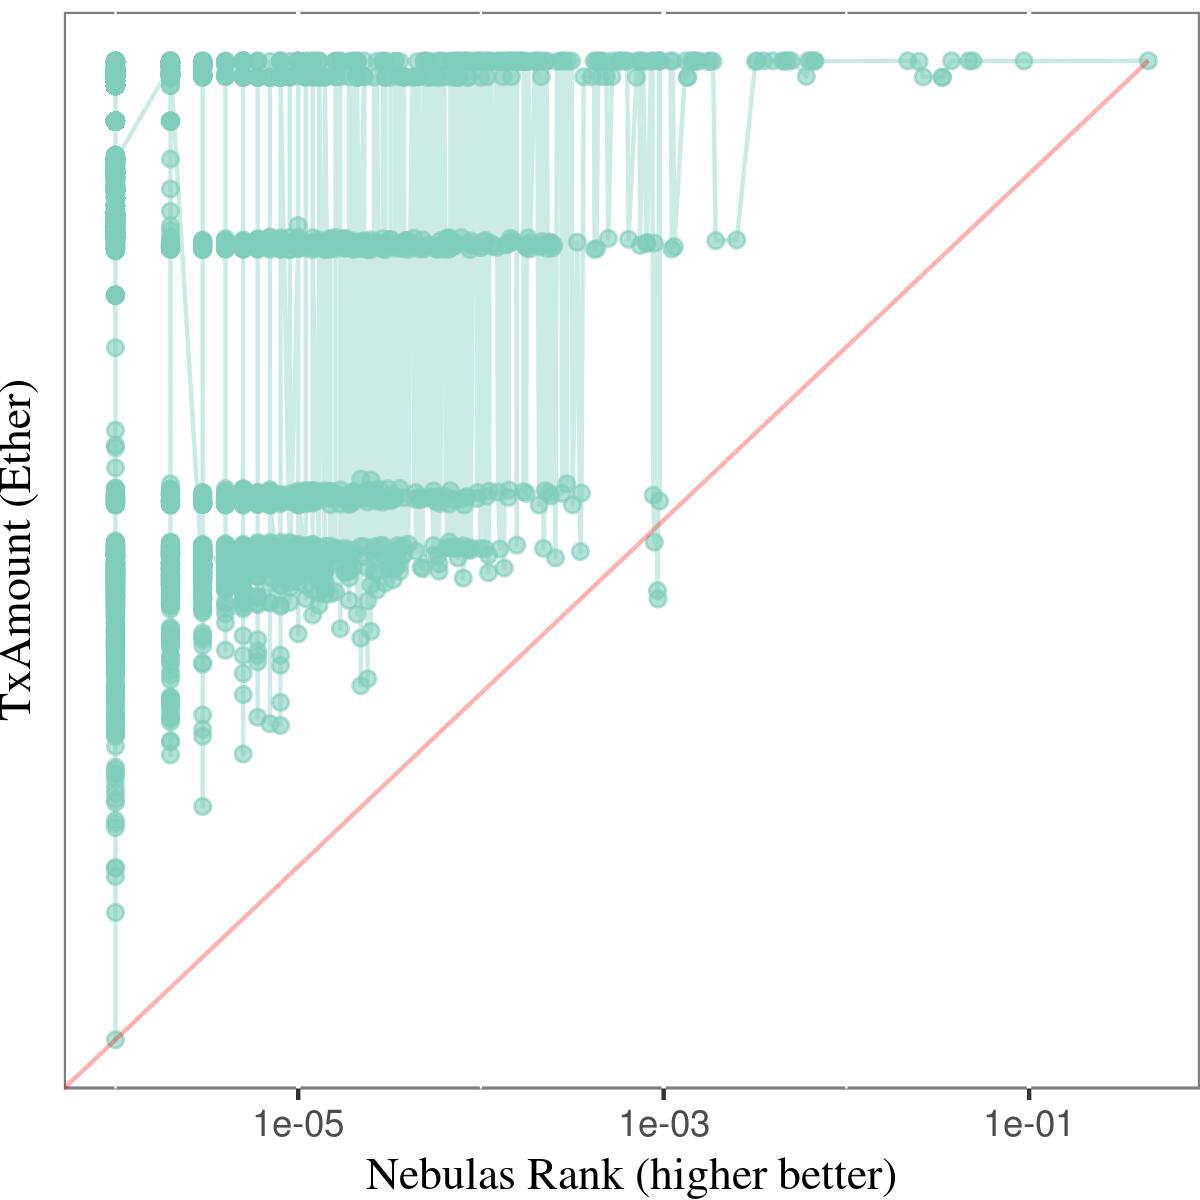
\includegraphics[width=0.50\textwidth]{figs/MAY_lr.png}
	\caption{Nebulas Rank versus monto de transacción \small{El eje de abscisas representa la valuación (\textit{rank value}), y el eje de ordenadas representa el monto de las transacciones; ambos ejes se presentan en escala logarítmica. La línea diagonal muestra que el monto de la transacción y la valuación son directamente proporcionales. Un buen algoritmo debe hacer que los puntos caigan lo menos posible en la parte inferior derecha de la diagonal, para evitar la existencia de nodos con transacciones de montos bajos y con alta valuación.}}\label{fig:nrio}
\end{figure}

De acuerdo con el simple análisis anterior, se puede deducir que los tres primeros tipos de manipulación pueden ser filtrados eficazmente por métodos específicos. Por lo tanto, finalmente, sólo necesitamos simular el último tipo y observar si se produce un efecto de resistencia. El atacante elige un nodo ligado a una casa de cambio de renombre para crear transferencias en bucle durante $X$ veces. Cada bucle de transferencia se compone de dos fases: primero el atacante transfiere $Y$ ETH a la casa de cambio a través de una nueva cuenta provisoria; luego el atacante recupera su dinero a través de otra dirección. La topología y el proceso atacantes se demuestran en la \reffig{fig:loop}. Este tipo de ataque explota el hecho de que el servicio de una casa de cambio está dispuesto a establecer vínculos con cualquier nodo a un costo muy bajo. Si bien es cierto que los nodos normales pueden realizar transferencias regulares con las casas de cambio, ninguno de estos casos mejoran la liquidez monetaria efectiva, y deben ser distinguidos de las operaciones normales.
\begin{figure}[!ht]
	\centering
	%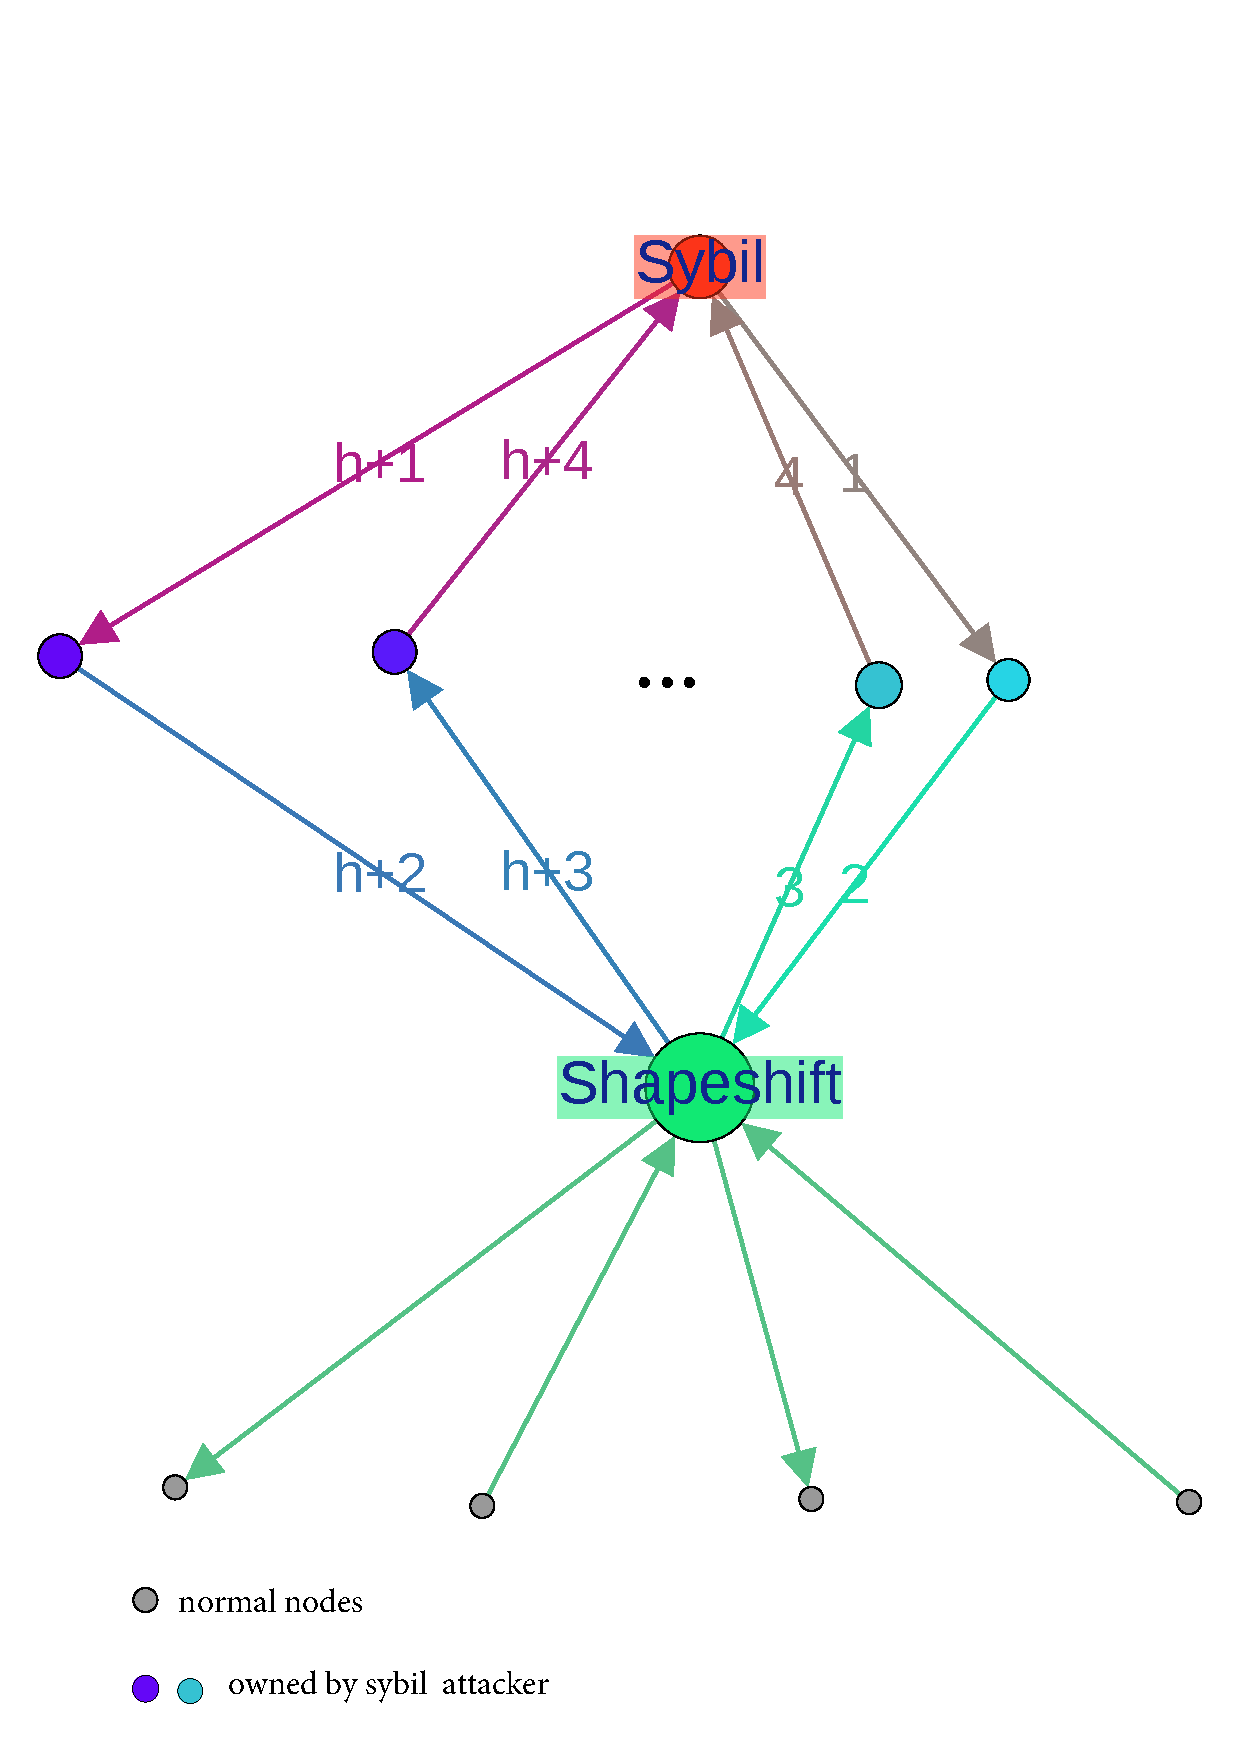
\includegraphics[width=0.35\textwidth]{figs/attack.pdf}
  \begin{tikzpicture}
  \pgfmathsetmacro{\YMD}{3}
  \pgfmathsetmacro{\XMD}{2}
\tikzset{
  hnode/.style={draw, circle, on grid, align=center, minimum height=2ex},
  base/.style={draw, circle, on grid, align=center, minimum height=4ex},
  sybil/.style={draw, circle, on grid, align=center, minimum height=4ex, fill=blue!20},
  normal/.style={draw, circle, on grid, align=center, minimum height=1ex, fill=gray!20},
  coord/.style={coordinate, on grid, node distance=6mm and 25mm},
}
%
\tikzset{>=stealth',
  every join/.style={->}, very thick}

       \node [base, fill=green!=20] (ss) at (0, 0) {} node[right
       = 1ex of ss] {Shapeshfit};

       \node (dot) at ($(ss.north) + (0, \YMD)$) {...};

       \node [sybil] (sy) at ($(dot.north) + (0, \YMD)$) {} node[right=1ex of
       sy]{Sybil};

       \node [hnode, fill=brown!50] (hh4) at($(dot.west) + (-\XMD, 0)$){};
       \node [hnode, fill=brown!50] (hh1) at ($(hh4.west) + (-\XMD, 0)$){};

       \node [hnode, fill=cyan!20] (h4) at ($(dot.east) + (\XMD, 0)$){};
       \node [hnode, fill=cyan!20] (h1) at ($(h4.east) + (\XMD, 0)$){} node
       [right = 1ex of h1]{owned by sybil attacker};

       \node [coord] (c) at($(ss.south) + (0, -\YMD)$) {};

       \node [normal] (n2) at ($(c.west) + (-\XMD, 0)$){};
       \node [normal] (n1) at ($(n2.west) + (-\XMD, 0)$){};
       \node [normal] (n3) at ($(c.east) + (\XMD, 0)$){};
       \node [normal] (n4) at ($(n3.east) + (\XMD, 0)$){} node [right=1ex of
       n4] {normal nodes};

       \draw[->, color=red] (sy) -- (hh1) node [midway, left]{4h+1};
       \draw[->, color=red] (hh4) -- (sy) node [midway, right]{4h+4};
       \draw[->, color=olive] (h4) -- (sy) node [midway, left]{4};
       \draw[->, color=olive] (sy) -- (h1) node [midway, right]{1};

       \draw[->, color=red] (hh1) -- (ss) node [midway, left]{4h+2};
       \draw[->, color=red] (ss) -- (hh4) node [midway, right]{4h+3};
       \draw[->, color=olive] (ss) -- (h4) node [midway, left] {3};
       \draw[->, color=olive] (h1) -- (ss) node [midway, right]{2};

       \draw[->] (ss) -- (n1);
       \draw[->] (n2) -- (ss);
       \draw[->] (ss) -- (n3);
       \draw[->] (n4) -- (ss);

\end{tikzpicture}

	\caption{Esquema de un ataque de bucle utilizando una dirección de casa de cambio \small{En la figura vemos el primer y el $h$-ésimo ataques de bucle. El nodo seleccionado pertenece a la casa de cambio Shapeshift; las etiquetas de las aristas indican la secuencia temporal; el monto transferido entre los nodos controlados por un atacante Sybil y el de Shapeshift es $Y$ ETH; Hay $X$ transferencias de bucle durante la manipulación.}}\label{fig:loop}
\end{figure}

Elegimos la dirección 0x70faa28a6b8d6829a4b1e649d26ec9a2a39ba413 que pertenece a la casa de cambio Shapeshift. Los resultados se muestran en la  \reffig{fig:antiManipulation}: 1) como se ve en la \reffig{subfig:deposit}, ningún algoritmo es capaz de prevenir que mejore la valuación del atacante cuando éste invierte más capital, mientras el grafo de transacciones definido en \refsec{subsec:txg} reduce los efectos del ataque. \textbf{Nebulas Rank} no sólo puede escoger nodos con un alto rendimiento de transacciones, sino que además resiste esta manipulación hasta cierto límite; 2) tal como se muestra en la \reffig{subfig:times}, con el atacante creando más transferencias en bucle, el grafo de transacciones definido en \refsec{subsec:txg} puede hacer que la valuación del atacante empeore; la razón para ello es que ese grafo toma en consideración factores como la \textit{antigüedad de los depósitos} y el valor \textit{estímulo}. Entretanto, \textbf{Nebulas Rank} podría fortalecer estos factores, generando así más resistencia contra la manipulación.

\begin{figure}[htbp]
	\centering
	\begin{subfigure}{\linewidth}
		\centering
		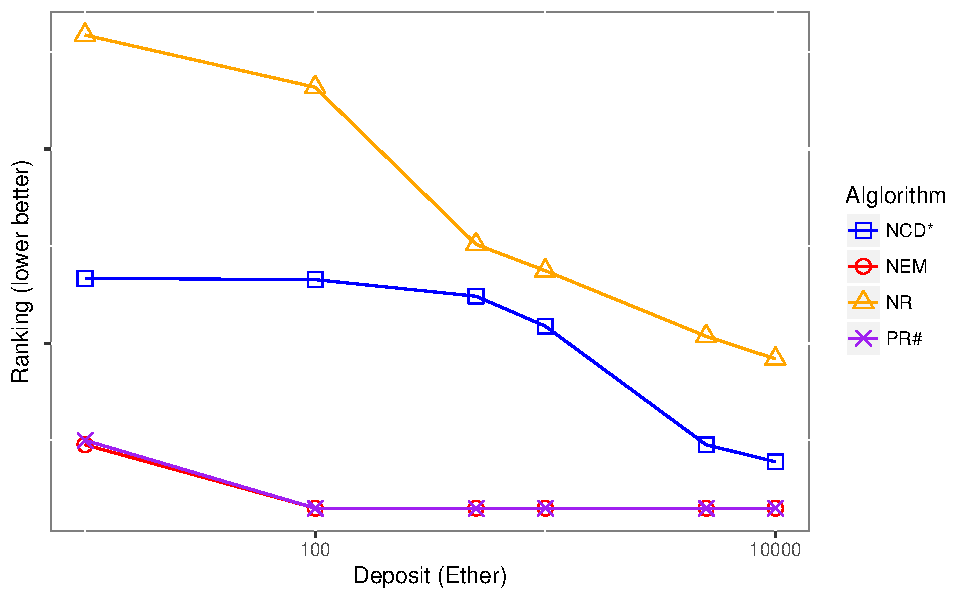
\includegraphics[width=0.7\textwidth]{figs/AttackDeposit.pdf}
		\caption{El efecto del tamaño del capital del atacante en su valuación, con el número de transferencias en bucle fijado en $5,000$. \small{(Los ejes están en escala logarítmica)}}
		\label{subfig:deposit}
	\end{subfigure}

	\begin{subfigure}{\linewidth}
	    \centering
		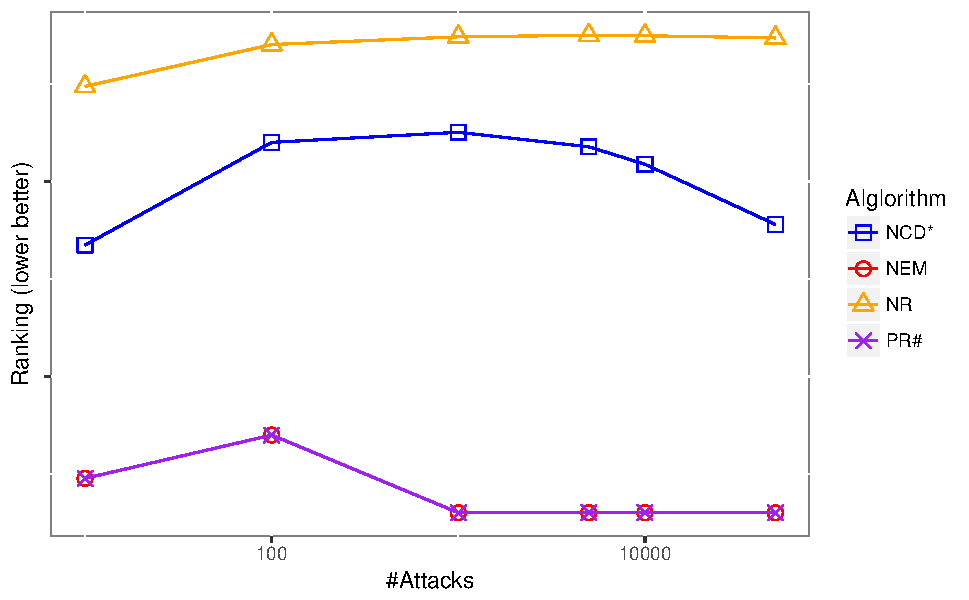
\includegraphics[width=0.7\textwidth]{figs/AttackTimes.pdf}
		\caption{El efecto del número de transferencias en bucle en la valuación del atacante, con su capital fijado en $\Xi5000$ \small{(Los ejes están en escala logarítmica)}}\label{subfig:times}
	\end{subfigure}

	\caption{Resistance contra la manipulación} \label{fig:antiManipulation}
	\caption*{\footnotesize{El método de ataque se muestra en la \reffig{fig:loop}; el eje de abscisas representa el capital del atacante, y el eje de ordenadas, el orden de su valuación (un orden de valuación mayor significa que el atacante falla en obtener mayor valuación, indicando una mayor resistencia por parte del algoritmo)  \\
	NR: el grafo de transacciones se define en \refsec{subsec:txg}, y el algoritmo de valuación se describe en \refsec{subsec:leaderrank}; \\
	%PR$^*$: The transaction graph is defined at \refsec{subsec:txg}, PageRank algorithm;\\
	NCD$^*$: el grafo de transacciones se define en \refsec{subsec:txg}, junto al algoritmo NCDawareRank; \\
	NEM: el grafo de transacciones es presentado por \cite{nem}, junto a NCDawareRank\\
	PR$^{\#}$: el grafo de transacciones es presentado por \cite{nem}, junto al algoritmo PageRank\\
	El factor de atenuación de PageRank es de 0,15; El algoritmo de clustering utilizado por NCDawareRank es pscan\cite{chang2017mathsf}, $\eta=0.75$, $\mu=0.1$}}
\end{figure}

\subsection{Trabajos relacionados} \label{subsec:related}

La centralidad, el índice de valuación base, es el concepto más estudiado en la ciencia de redes desde hace décadas\cite{newman2010networks}. Hay un cuerpo de literaturas que introducen varias centralidades, incluyendo la centralidad de los grados\cite{freeman1979set}, la centralidad de los valores propios\cite{bonacich1972factoring}, la centralidad de Katz\cite{katz1953new}, la centralidad de cercanía\cite{sabidussi1966centrality}, la centralidad intermedia\cite{freeman1977set}\cite{freeman1978centrality}\cite{freeman1991centrality}\cite{noh2004random}\cite{newman2005measure}, PageRank\cite{Brin2010}, HITS\cite{kleinberg1999authoritative}, SALSA\cite{Science2001}, etc.

Además, hay algunos trabajos fundamentales que tratan de clasificar y revisar claramente estas medidas mediante un marco de trabajo unificado\cite{Borgatti2005}\cite{Borgatti2006}\cite{Lu2016}. Al diseñar \textbf{Nebulas Rank}, antes de adoptar centralidad, primero es necesario considerar la propiedad del grafo. El escenario del grafo de transacciones de blockchain es mayormente similar a la red de flujos monetarios mencionada en \cite{Borgatti2005}. Sin embargo, los algoritmos relacionados mencionados por su trabajo —tales como flujo de centralidad intermedia\cite{freeman1991centrality} y paseo aleatorio de centralidad intermedia (también conocido por \textit{current betweenness centrality})\cite{newman2005measure}— son intensivos en computación y no satisfacen la propiedad \textit{computable} en la gran escala del grafo de transacciones de Blockchain.

Desde el lanzamiento de Bitcoin\cite{Nakamoto2008} en 2009, los investigadores han realizado algunos análisis estadísticos y empíricos sobre el grafo de transacciones de Bitcoin\cite{Ron}\cite{Haslhofer}\cite{NielKondor2014}\cite{Baumann2014}, y algunos de ellos utilizan la estructura del grafo de transacciones para discutir el anonimato de esa red\cite{Meiklejohn2013}\cite{Ober2013}\cite{pham2016anomaly}\cite{Fleder2015}\cite{Ferrin2015}. Después del lanzamiento y popularización de otras criptodivisas, se llevó a cabo un análisis del grafo de transacciones sobre más blockchains\cite{Chang2017}\cite{Anderson2016}. \textbf{Nebulas Rank} adopta sus conceptos de grafos de transacciones; esto es, Grafo de Entidades en \cite{Tschorsch2015}, con algunas revisiones menores. Es decir, cada cuenta, o conjunto de cuentas que pertenecen a la misma gente, se mapea como un nodo, y cada arista dirigida representa la intensidad de la transferencia entre dos cuentas. En realidad, antes de que se inventara un sistema blockchain como Bitcoin, los científicos intentaron estudiar algunas redes financieras entre bancos y entidades de comercio mundial.\cite{propper2008towards}\cite{Boss2004}\cite{Serrano2007}\cite{Bech2008}\cite{Fagiolo2009}\cite{Morten2006}\cite{Boss2004a}\cite{Krempel2002}\cite{Serrano2003}. Comparando con el grafo de transacción en blockchain, estas redes financieras estudiadas tempranamente se definen no sólo por la transferencia de actividades, sino también por información adicional (como préstamos). Además, la escala de esas redes es mucho menor. Para concluir, rara vez se han realizado trabajos de investigación que propongan un método de valuación personalizado para un grafo de transacción a gran escala, especialmente un grafo de transacciones en el blockchain.

El trabajo más relevante con \textbf{Nebulas Rank} es el esquema de Prueba de Importancia NEM\cite{nem}. Éste adopta NCDawareRank\cite{Nikolakopoulos2013}, que explota el efecto de clustering de la topología de red, como el algoritmo de valuación, con su algoritmo de clustering basado en el de SCAN\cite{xu2007scan}\cite{shiokawa2015scan}\cite{chang2017mathsf}. Aunque la estructura de comunidad existe en el grafo de transacción y debería ser útil para manejar los nodos de spam, no se garantiza que todos los nodos en el mundo Blockchain, controlados por una entidad en el mundo real, estén mapeados en un solo cluster, lo que deja mucho espacio para la manipulación. Además, \cite{Fleder2015} utiliza PageRank\cite{Brin2010}\cite{page1999pagerank} como métrica auxiliar para el descubrimiento de direcciones interesantes, y para el análisis de sus actividades. No obstante ello, su trabajo no brinda un marco de trabajo automatizado para la identificación de nodos importantes. En vez de ello, éste depende del análisis subjetivo, lo que no concuerda con el contexto de \textbf{Nebulas Rank}.

El algoritmo que elegimos es LeaderRank\cite{Chen2013}\cite{Li2014}. Es una variante simple pero efectiva de PageRank\cite{Brin2010}\cite{page1999pagerank}; en ésta, cada nodo tiene asignado un parámetro de teleportación idéntido, mientras LeaderRank agrega un llamado \textit{nodo ground}, asignándole distintos parámetros de teleportación por cada nodo. El esquema de ponderación de \textbf{Nebulas Rank} está tomado parcialmente del diseño de \cite{Li2014}, lo que permite que los nodos con mayor grado de ingresos tengan más chances de teleportación. Adoptar el algoritmo LeaderRank podría arrojar resultados más afines al escenario de Blockchain.